% Contributors: Alexandre Lamy, Trung Vu
\section{The watershed algorithm}
  The watershed algorithm is another density based clustering method, often used in image classification.
  The algorithm has two steps. First it estimates the density of the distribution over the space (i.e. 
  it estimates the probability density function (PDF) of the distribution from which it assumes that the data points
  have been drawn). We will see exactly how this can be done in later sections. 
  
  Then the algorithm will ``flip'' the estimated PDF and start ``filling it with water''. Regions where water from different
  ``wells'' touch for the first time will become cluster boundaries.
  
  Figure \ref{watershed} shows the boundaries formed by the watershed algorithm on a toy 1 dimensional PDF.
  
  \begin{figure}[h]
  \centering
  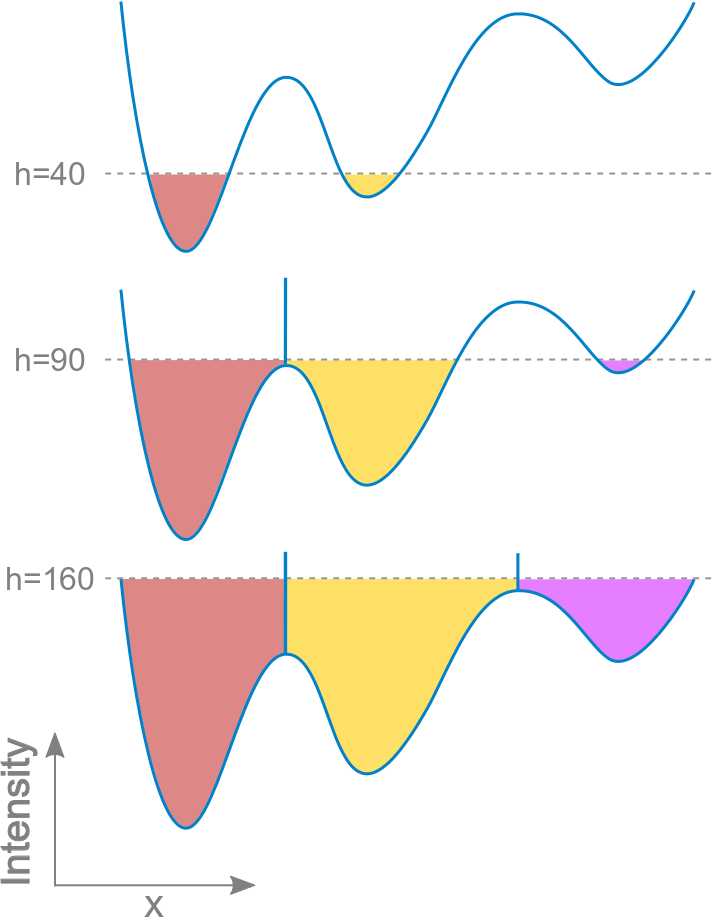
\includegraphics[width=.3\linewidth]{chapter_2/files/Watershed-flooding-graph.png}
  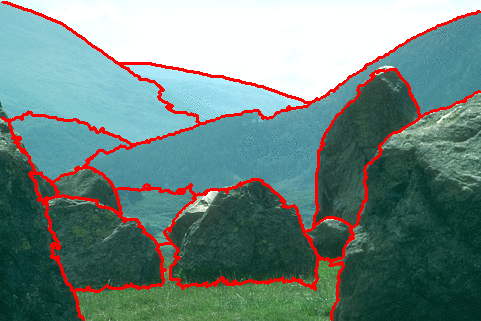
\includegraphics[width=.6\linewidth]{chapter_2/files/PW_overlay.png}
  \caption{Watershed algorithm applied to a 1D PDF (left) and to a 2D image (right) }
  \label{watershed}
  \end{figure}
  
  The watershed algorithm is often used for image recognition tasks. The idea is that rather than 
  analyzing each pixel (i.e. making each pixel a feature and then running some classification algorithm)
  one can first cluster the pixels to form very similar ``meta-regions''. These, rather than the individual pixels,
  can then be made into features of the image for further tasks. Figure \ref{watershed} shows the results one can
  obtain by running watershed on a 2d image.
  
